\clearpage
\item \subquestionpoints{10} \textbf{Coding problem.}
Using the validation set, estimate the constant $\alpha$ by averaging your
classifier's predictions over all labeled examples in the validation set:
%
\begin{equation*}
  \alpha \approx \frac{1}{|V_{+}|}\sum_{x^{(i)}\in V_{+}} h(x^{(i)}).
\end{equation*}
%
Add code in \texttt{src/p02cde\_posonly.py} to rescale your
classifier's predictions from part (d) using the estimated value for $\alpha$.

Finally, using a threshold of $p(t^{(i)} = 1 \mid x^{(i)}) = 0.5$, make three
separate plots with the decision boundaries from parts (c) - (e) plotted on top
of the test set. Plot $x_1$ on the horizontal axis and $x_2$ on the vertical
axis, and use two different symbols for the positive ($t^{(i)} = 1$) and
negative ($t^{(i)} = 0$) examples. In each plot, indicate the separating
hyperplane with a red line.

\ifnum\solutions=1 {
  \begin{answer}
    \begin{figure}[htbp]
        \centering
        \begin{minipage}[t]{0.48\textwidth}
        \centering
        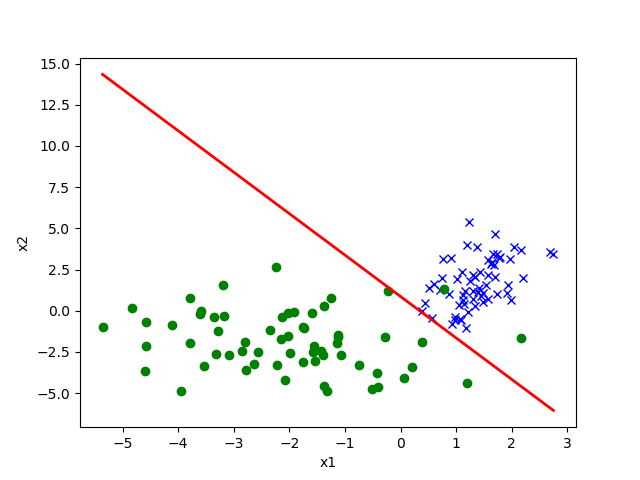
\includegraphics[width=6cm]{../src/output/p02c_pred.png}
        \caption{train and test on true labels}
        \end{minipage}
        \begin{minipage}[t]{0.48\textwidth}
        \centering
        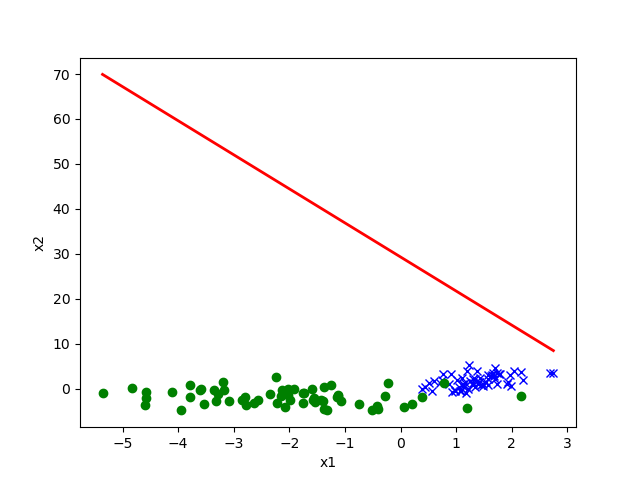
\includegraphics[width=6cm]{../src/output/p02d_pred.png}
        \caption{train on y labels, test on true lables}
        \end{minipage}
        \begin{minipage}[t]{0.48\textwidth}
        \centering
        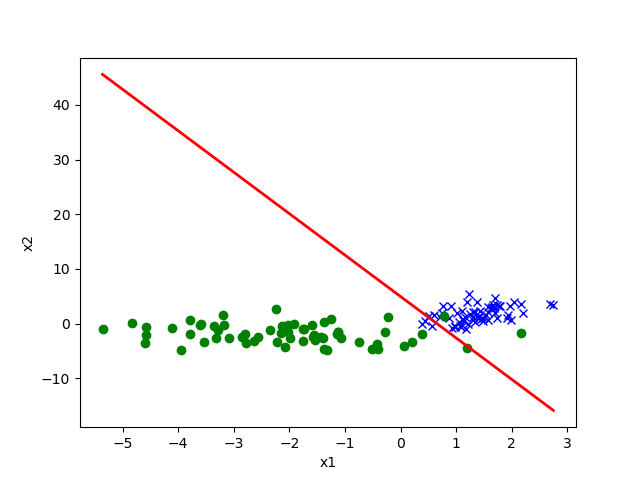
\includegraphics[width=6cm]{../src/output/p02e_pred.png}
        \caption{rescale by alpha}
        \end{minipage}
    \end{figure}
\end{answer}

} \fi
